\documentclass[assd_tp2_main.tex]{subfiles}

\begin{document}

\section{Síntesis de sonidos mediante modelos f\'isicos}
Se analizarán dos variantes del modelo Karplus-Strong en paralelo, tanto de manera teórica como práctica. 

\subsection{Bloque A Elemental}
Se resolverá, como cálculo auxiliar un bloque sencillo definido como:
\begin{figure}[H]	
	\centering
	\includegraphics[scale=1]{graficos/bloque1ej5.png}
	\caption{Bloque elemental}
	\label{fig:bloqueElemental}
\end{figure}

Este bloque solo promedia los dos ultimos valores de entrada. Su transferencia esta dada por
\begin{equation}
x(n)=\frac{1}{2}x(n)+\frac{1}{2}x(n-1)
\end{equation}
\begin{equation}
Y(z)=\frac{1}{2}X(z)+\frac{1}{2}X(z)z^{-1} \implies A(z)=\frac{z+1}{z}
\end{equation}
Se puede observar que el bloque A es pasa-bajos (cero en $Z=-1$); lo cual es, en principio, razonable, el bloque A suaviza la entrada.

\subsection{Karplus Strong 1}
\subsubsection{Análisis teórico}
Se resolverá un nuevo sistema, denominado $S_1$, el cuál consiste en una adicion de realimentación al sistema anterior.
\begin{figure}[H]	
	\centering
	\includegraphics[scale=1]{graficos/bloque2ej5.png}
	\caption{Bloque elemental}
	\label{fig:bloqueElemental}
\end{figure}

Mediante teoria de feedback a considerando que $B(z)=z^{-L}R_L$ se llega a que
\begin{equation}
S_1(z)=\frac{ \frac{1}{2} z^{L+1} + \frac{1}{2}z^L}{ z^{L+1} - \frac{1}{2}R_L z-\frac{1}{2}R_L } 
\end{equation}

Es decir, una expresión con $L+1$ polos y $L+1$ ceros, en otras palabras, una ecuación diferencial de orden $L+1$ con vector de longitud $L$ como condición inicial.

\subsubsection{Estudio de la distribución polos y ceros, respuesta en frecuencia}
\begin{figure}[H]	
	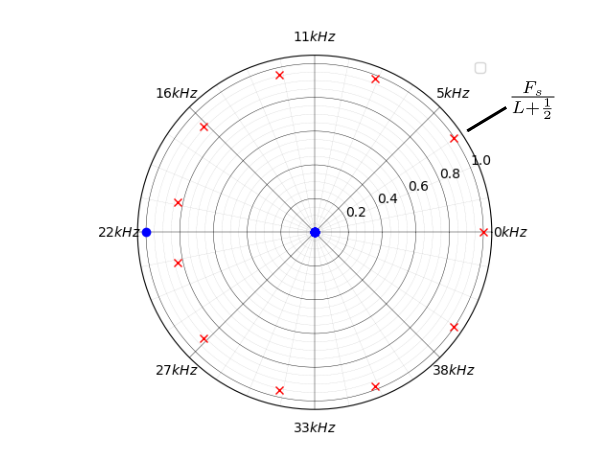
\includegraphics[scale=0.45]{graficos/polos.png}
	\includegraphics[scale=0.58]{graficos/freq_response.png}
	\caption{Polos y ceros (derecha), Rta en frecuencia (izquierda), $S_1$ con $R_L=1$, $L=10$, $f_s=44.1kHz$}
	\label{fig:polosCeros}
\end{figure}

Del diagrama de polos y ceros y la respuesta en frecuencia podemos observar que hay una frecuencia de resonancia $F_R=F_s/(L+\frac{1}{2})$ que tiende a cumplir las hipotesis del criterio de Barkhausen, y por lo tanto provocar oscilaciones, lo cuál es el objetivo del bloque; conseguir una salida que perdure en el tiempo a partir de una entrada de longitud $L$ muy corta.

\subsubsection{Cálculo de $F_R$}
Se mostrará porque el sistema resuena en $F_r=F_s/(L+\frac{1}{2})$. En la sección anterior se observó que la frecuencia de resonancia debía ser aquella que tendiera a cumlir las hipotesis del criterio de barkhausen; en otras palabras; que la ganancia del lazo se aproxime a $1\phase 0$

\subsubsection{Análisis de estabilidad}

Se estudiaran condiciones para garantizar la estabilidad del sistema

\subsubsection{Análisis mediante señales}
 
Se procederá a estudiar como el sistema responde a diversas entradas, entre ellas, un impulso unitario, ruido gaussiano de longitud $L$, y ruido lineal de longitud $L$. Se decidió aumentar $L$ en estos casos a $50$ para conseguir frecuencias más cercanas a las audibles.
 
\begin{figure}[H]
	\includegraphics[scale=0.55]{graficos/impulsoBloqueS1.png}
	\includegraphics[scale=0.41]{graficos/impulsoBloqueS1Zoom.png}
	\caption{Respuesta al impulso con y sin zoom, $R_L=1$, $L=50$, $f_s=44.1kHz$}
\end{figure}

Se puede observar que, de todas las frecuencias pertenecientes al impulso, la más amplificada vale $865Hz \approx \frac{F_s}{1/2+L}$. Por otro lado es importante observar que la salida se encuentra montada sobre una tensión continua, más precisamente, nunca es menor que 0. Esto se debe a que cuando la excitación es exclusivamente positiva, como la realimentación es positiva y no hay inversiones la salida siempre será positiva. Por ello es importante que la excitación inicial sea tanto positiva como negativa para lograr que la salida este centrada en 0.

\begin{figure}[H]
	\includegraphics[scale=0.55]{graficos/gaussBloqueS1.png}
	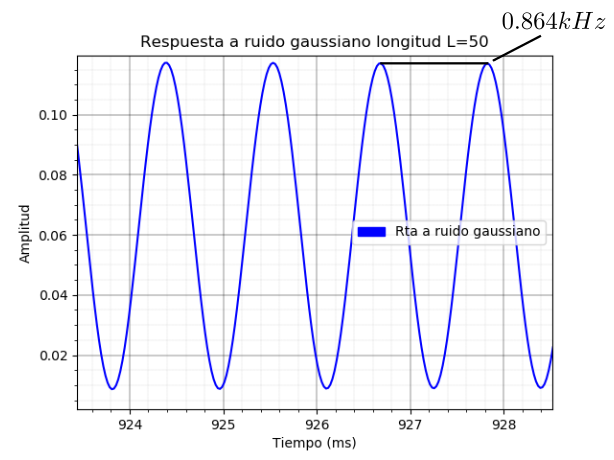
\includegraphics[scale=0.41]{graficos/gaussBloqueS1zoom.png}
	\caption{Respuesta a entrada Gaussiana con y sin zoom, $R_L=1$, $L=50$, $f_s=44.1kHz$}
\end{figure}

Se puede ver que la salida fue a la misma frecuencia que en el caso anterior, al mismo tiempo que nuevamente, estuvo montada sobre una continua. No obstante la salida tuvo la posiblidad de tomar valores negativos.

\begin{figure}[H]
	\includegraphics[scale=0.55]{graficos/randomBloqueS1.png}
	\includegraphics[scale=0.55]{graficos/randomBloqueS1zoom.png}
	\caption{Respuesta a entrada Gaussiana con y sin zoom, $R_L=1$, $L=50$, $f_s=44.1kHz$}
\end{figure}

\subsection{Karplus Strong 2}

\subsubsection{Analisis teórico elemental}
Se estudiará un nuevo sistema con una pequeña modificación la cual consiste en agregar un multiplicador en el bloque realimentador, cuyo valor es aleatorio entre -1 y 1
Escrito en lenguaje matemático

\begin{equation}
	A(z)=b(\frac{1}{2}+\frac{1}{2}z^{-1})
\end{equation}
\begin{equation}
	B(z)=\frac{1}{2}z^{-l}
\end{equation}

Usando teória de feedback concluimos que

\begin{equation}
	H(z)=\frac{\frac{1}{2}b+\frac{1}{2}bz^{-L}}{1-\frac{1}{2}bR_Lz^{-L}-b\frac{1}{2}R_Lz^{-L-1}}
\end{equation}

\subsubsection{Cálculo $\phi(w)$}


\subsubsection{Cálculo de $F_R$}
Se procederán a realizar los cálculos para conseguir la frecuencia de resonancia del sistema.

\end{document}

